\chapter{Analisa Masalah}
\label{chap:analisa}

	Pada bab ini akan dibahas mengenai hasil analisa permasalahan flow shop dan segalah hal yang berkaitan dengan analisa permasalahan tersebut.
	Pada bab ini juga akan dibahas sekilas mengenai rancangan awal dari perangkat lunak yang memungkinkan diaplikasikannya
	algoritma ant colony pada permasalahan multi objective flow shop.
	
	
\section{Analisa Kasus}

	Proses penjadwalan Flow Shop adalah salah satu metode penjadwalan produksi di mana urutan mesin 
	yang digunakan untuk setiap proses dalam seluruh pekerjaan harus sama. Pekerjaan-pekerjaan tersebut
	akan dikerjakan pada mesin-mesin yang ada dengan urutan pengerjaan yang dipilih. Masing - masing
	proses akan dikerjakan secara sistematis dan terurut. Data-data masukan yang dibutuhkan
	dalam menjalankan sebuah proses penjadwalan flow shop adalah:
	\begin{itemize}
		\item Banyaknya pekerjaan
		\item Banyaknya mesin
		\item Detail waktu pengerjaan setiap pekerjaan
		
	\end{itemize}

	Setiap pekerjaan memiliki waktu proses yang berbeda satu sama lain pada tiap mesin. Variasi
	urutan pengerjaan yang berbeda biasanya akan menghasilkan waktu pengerjaan / makespan yang
	berbeda pula. Proses penjadwalan ini penting untuk diperhatikan, karena mampu mempengaruhi
	lama waktu penggunaan fasilitas dalam suatu proses produksi. Urutan pengerjaan yang baik dapat
	dicari dengan menggunakan suatu algoritma optimisasi. Diharapkan dengan algoritma optimisasi
	tersebut, urutan pengerjaan yang menghasilkan makespan / waktu pengerjaan minimum dapat
	ditemukan.
	
	Salah satu algoritma yang dapat digunakan untuk optimisasi penjadwalan flow shop
	adalah algoritma ant colony. Tingkat keoptimalan setiap algoritma berbeda-beda, oleh karena
	itu perlu dibuat sebuah perangkat lunak untuk optimisasi penjadwalan flow shop dengan
	menggunakan algoritma ant colony. Algoritma ant colony akan menerima data masukan dari suatu
	kasus flow shop, kemudian akan mencari urutan pengerjaan / solusi yang paling optimal dari
	kasus tersebut selain itu kita juga dapat mencari kriteria lain yang kita inginkan.
	
	Algoritma ant colony akan mencari urutan pengerjaan yang menghasilkan makespan / waktu
	pengerjaan yang paling minimum. Algoritma ant colony merepresentasikan pilihan solusi-solusi
	yang ada sebagai jalur yang akan dilalui oleh semut dan memberikan data feromon sebagai panduan
	untuk melewati jalur-jalur tersebut. Dengan panduan tersebut, semut-semut tersebut diasumsikan
	mampu memilih jalur yang paling optimal.
	Proses optimisasi dengan menggunakan algoritma ant colony perlu memperhatikan beberapa
	hal. 
	
	Algoritma ant colony perlu mengetahui bagaimana cara merepresentasikan suatu solusi sebagai 
	jalur, bagaimana cara menggunakan panduan feromon untuk pemilihan jalur, bagaimana cara
	membaca dan menyimpan suatu data feromon, serta banyak hal lainnya. Tata cara tersebut mampu
	mempengaruhi hasil optimisasi dari algoritma ant colony.
	
\section{Analisa Algoritma Ant Colony Pada Penjadwalan Flow Shop}

\subsection{Urutan Pengerjaan Proses Sebagai Jalur Semut}
	Algoritma ant colony akan membantu penentuan urutan pengambilan pekerjaan yang optimal. Oleh
	karena itu, algoritma ini akan merepresentasikan pilihan urutan pengambilan yang ada sebagai jalur. 
	Jalur-jalur tersebut kemudian akan dilewati oleh semut-semut yang akan mencari solusi / urutan pengerjaan 
	yang optimal. Pilihan urutan pengerjaan yang ada dapat dicari dengan menggunakan fungsi permutasi terhadap 
	jumlah pekerjaan.

	Sebagai contoh, jika dimisalkan terdapat 3 buah pekerjaan, maka dengan fungsi permutasi akan
	didapatkan jalur-jalur urutan pengerjaan (1,2,3), (1,3,2), (2,1,3), (2,3,1), (3,1,2), dan (3,2,1). Fungsi
	permutasi ini digunakan dengan mempertimbangkan sifat dari proses penjadwalan flow shop.
	Masing-masing proses dari pekerjaan pasti akan dikerjakan dan hanya akan dikerjakan sebanyak
	satu kali.

\subsection{Memilih Urutan Pengerjaan / Jalur}
	Makespan yang dihasilkan oleh masing-masing urutan pengerjaan biasanya akan bernilai berbeda.
	Penentuan urutan pengerjaan yang optimal akan ditentukan oleh nilai feromon yang akan diberikan
	oleh semut-semut yang telah disebar. Nilai feromon tersebut dapat disimpan dengan cara yang
	beragam.

	Dalam kasus flow shop juga terdapat beragam cara dalam menyimpan feromon dan
	penentuan urutan yang lebih optimal. Salah satunya adalah dengan menyimpan nilai feromon
	sebagai panduan pemilihan pekerjaan selanjutnya. Nilai feromon akan menyimpan kecenderungan
	dipilihnya suatu pekerjaan setelah dipilihnya suatu pekerjaan yang lain. Nilai feromon tersebut
	akan disimpan dalam bentuk matriks 2 dimensi.

	Indeks pertama dari matriks akan merepresentasikan nomor pekerjaan yang sebelumnya dipilih.
	Indeks kedua akan merepresentasikan pekerjaan yang selanjutnya akan dipilih. Sebagai contoh,
	pada matriks indeks [1][2] menunjukkan kecenderungan dipilihnya pekerjaan 2 setelah dipilihnya
	pekerjaan 1. Nilai feromon pada matriks dengan 2 indeks yang sama akan selalu bernilai 0.

	Perlu diingat pula bahwa algoritma ant colony akan selalu memberikan peluang dipilihnya sebuah
	solusi. Meskipun solusi tersebut sudah dapat dianggap sebagai solusi yang kurang optimal,
	solusi tersebut harus tetap memiliki kemungkinan untuk dipilih. Oleh karena itu, indeks nilai feromon
	harus tetap dapat mengacu pada terpilihnya suatu solusi-solusi yang ada. Nilai feromon
	masing-masing indeks matriks (kecuali matriks dengan dua indeks yang sama) tidak akan lebih kecil
	dari 1. Hal ini dilakukan agar setiap solusi masih memiliki kemungkinan untuk dipilih, meskipun
	kemungkinannya sangat kecil.

\subsection{Proses Pemilihan Urutan Pengerjaan / Jalur Semut}
	Pada proses pemilihan jalur, nilai feromon yang disimpan oleh suatu indeks matriks mempengaruhi
	kemungkinan dipilihnya suatu pekerjaan. Semakin besar nilai feromon pada suatu indeks, semakin
	besar kemungkinan dipilihnya pekerjaan yang dirujuk oleh indeks matriks tersebut. Berdasarkan
	rumus untuk pemilihan jalur pada algoritma ant colony, diperlukan nilai objektif dan nilai feromon
	untuk penentuan pemilihan suatu jalur. Pada proses pemilihan pekerjaan ini, nilai objektif
	yang digunakan adalah 1 untuk semua indeks matriks. Proses pemilihan pekerjaan ini hanya akan
	dipengaruhi oleh nilai feromon yang disimpan pada indeks matriks yang ada.

	Penentuan pekerjaan mana yang akan dipilih dapat dimulai dengan melakukan proses randomisasi
	suatu angka. Angka tersebut akan berada di kisaran nilai 1 hingga jumlah nilai feromon
	dari indeks-indeks yang mungkin dilibatkan. Penentuan pekerjaan dilakukan dengan menambahkan
	secara satu per satu nilai feromon dari indeks yang terlibat dimulai dari nilai 0. Jika setelah
	ditambahkan nilai dari suatu indeks, jumlah nilai telah melebihi angka hasil randomisasi, maka
	pekerjaan yang dirujuk indeks tersebut akan dipilih sebagai pekerjaan yang diambil.


	Proses pemilihan jalur dilakukan secara bertahap, dimulai dari pemilihan jalur pertama. Untuk
	pemilihan jalur pertama, nilai feromon yang mempengaruhi terpilihnya suatu jalur merupakan
	jumlah nilai feromon pada matriks dengan indeks kedua yang merujuk pada jalur tersebut. Sebagai
	contoh, jika dimisalkan terdapat 2 buah pekerjaan, maka jumlah nilai matriks pada indeks [1][1]
	dan indeks [2][1] merupakan nilai feromon untuk terpilihnya pekerjaan 1 untuk dikerjakan pertama
	kali.

	Untuk pemilihan pekerjaan selanjutnya dilakukan dengan representasi normal dari matriks tersebut.
	Indeks pertama berfungsi sebagai penunjuk pekerjaan yang diambil sebelumnya dan indeks
	kedua merupakan penunjuk pekerjaan yang akan diambil selanjutnya. Proses pemilihan ini akan
	memperhatikan pekerjaan-pekerjaan yang sebelumnya telah dipilih. Sebagai contoh, jika dimisalkan
	terdapat 4 buah pekerjaan dan urutan pekerjaan yang sudah dipilih adalah [1,2], maka indeks matriks
	yang akan diperhatikan dalam proses pemilihan hanya indeks matriks [2][3] dan [2][4]. Indeks
	matriks [2][1] tidak diperhatikan karena sudah diambil untuk dikerjakan pertama kali.


\subsection{Proses Penambahan Feromon}

	Setiap solusi yang dicoba akan menghasilkan makespan yang berbeda-beda. Nilai makespan yang
	dihasilkan mempengaruhi tingkat keoptimalan dari solusi tersebut. Semakin kecil nilai makespan
	yang dihasilkan, semakin besar tingkat keoptimalan dari suatu solusi.

	Nilai feromon yang disimpan harus mampu mempengaruhi semut-semut untuk lebih sering memilih
	jalur yang lebih optimal. Oleh karena itu, nilai feromon pada solusi optimal harus lebih cepat
	bertambah. Hal tersebut dapat dilakukan dengan memanipulasi banyak feromon yang ditambahkan.
	Semakin kecil nilai makespan yang dihasilkan, semakin besar nilai feromon yang akan disimpan
	atau ditambahkan.

	Nilai feromon yang akan ditambahkan merupakan hasil proses pengurangan antara nilai ma-
	kespan yang dihasilkan dengan suatu nilai tetap. Nilai tetap yang akan digunakan merupakan salah
	satu nilai makespan yang dihasilkan dari solusi yang akan dianggap sebagai nilai tengah dari ma-
	kespan yang mungkin dihasilkan. Solusi yang akan dijadikan nilai tengah ini merupakan solusi yang
	menggunakan urutan nama / nomor pekerjaan sebagai urutan pengerjaan. Sebagai contoh, jika
	terdapat 3 buah pekerjaan, maka solusi yang dijadikan nilai tengah adalah solusi dengan urutan
	pengerjaan [1,2,3].

	Banyaknya feromon yang ditambahkan tidak akan bernilai negatif. Jika feromon yang ditambahkan
	bernilai negatif, maka penambahan feromon dari solusi tersebut tidak akan dilakukan. Penambahan
	feromon akan dilakukan pada indeks-indeks matriks tertentu berdasarkan solusi yang
	diambil. Sebagai contoh, jika solusi yang diambil adalah [2,1,3], maka indeks-indeks matriks yang
	akan ditambahkan feromonnya adalah indeks matriks [2,1] dan [1,3]. Dengan ditambahkannya
	matriks pada indeks-indeks tersebut, diharapkan indeks matriks tersebut akan lebih sering diacu
	dalam proses pengambilan jalur. Dengan ditambahkannya feromon pada indeks-indeks tersebut
	juga diharapkan solusi dengan urutan pengerjaan [2,1,3] akan lebih sering diambil.



\section{Proses Optimisasi Penjadwalan Flow Shop Dengan Menggunakan Algoritma Ant Colony}

	Pada saat melakukan proses optimisasi, algoritma ant colony akan melakukan proses pelatihan
	secara berulang-ulang. Pada setiap proses pelatihan, algoritma ant colony menyebarkan sejumlah
	semut yang akan mengerjakan kasus flow shop sesuai solusi yang dipilih masing-masing
	semut. Solusi-solusi tersebut dipilih secara acak berdasarkan nilai feromon yang disimpan. Solusi solusi
	terbaik yang telah dipilih oleh suatu semut akan disimpan dan dibandingkan dengan solusi
	terbaik dari proses pelatihan sebelumnya.
	
	Penambahan dan evaporasi nilai feromon yang disimpan akan dilakukan setiap suatu fase pelatihan
	dari algoritma ant colony selesai dilakukan. Nilai feromon yang ditambahkan akan disesuaikan
	dengan solusi dan hasil yang didapat oleh masing-masing semut. Semakin baik hasil yang diberikan
	suatu solusi, semakin banyak nilai feromon yang ditambahkan pada indeks feromon yang mengacu
	pada solusi tersebut. Proses pelatihan akan terus dilakukan hingga suatu kondisi berhenti dicapai.
	Kondisi berhenti tersebut merupakan penanda bahwa hasil solusi yang dipilih sudah dapat dianggap
	sebagai solusi yang optimal.
	
	Algoritma ant colony merupakan algoritma optimisasi yang cukup terkenal. Keunggulan-keunggulan
	dari algoritma ini diantaranya adalah :
	\begin{itemize}
		\item Mampu diaplikasikan pada berbagai macam permasalahan.
		\item Mampu memberikan salah satu solusi yang dapat dianggap baik secara cepat.
	\end{itemize}

	Sedangkan kekurangan algoritma ini adalah :
	\begin{itemize}
		\item Solusi terbaik pasti ditemukan, akan tetapi tidak ada lama waktu yang pasti untuk ditemukannya
		solusi optimal tersebut.
		\item Analisa secara teori tidak mungkin dilakukan, karena menggunakan pengambilan solusi secara
		acak dan tidak tetap.
	\end{itemize}

	Untuk menangani kelemahan-kelemahan tersebut, algoritma ant colony perlu menjabarkan jumlah
	pelatihan yang akan dilakukan dan banyaknya semut yang akan disebar pada satu kali proses
	pelatihan. Hal-hal tersebut perlu ditentukan agar proses pelatihan mampu menemukan solusi yang
	optimal dalam waktu yang relatif cepat. Semakin banyak proses pelatihan dan jumlah semut yang
	disebar, semakin besar kemungkinan ditemukannya solusi yang optimal. Akan tetapi pada saat
	yang bersamaan akan meningkatkan waktu pelaksanaan proses optimisasi. Baik atau tidaknya suatu
	proses optimisasi ditentukan oleh tingkat keoptimalan solusi yang dihasilkan dan waktu yang
	diperlukan untuk proses optimisasi.
	
	\subsection{Jumlah Semut}
	
	Jumlah semut dalam proses optimisasi algoritma ant colony sangat berpengaruh pada tingkat keoptimalan
	dari solusi yang dihasilkan. Semakin banyak jumlah semut yang disebar, maka tingkat
	keoptimalan solusi yang diberikan akan cenderung lebih baik. Akan tetapi semakin banyak semut
	yang disebar akan menambah tingkat kompleksitas algoritma ini dan menambah waktu yang diperlukan
	untuk proses optimisasi. Jumlah semut yang disebar perlu ditentukan agar algoritma mampu
	memberikan solusi yang dapat dianggap cukup baik dalam waktu yang relatif cepat.
	
	Pencarian solusi optimal untuk suatu kasus flow shop dapat dilakukan secara brute force.
	Pencarian solusi secara brute force dapat dianggap sebagai cara yang paling tidak efisien. Brute
	force akan menjabarkan solusi-solusi yang ada dan mencoba penyelesaian dengan menggunakan
	masing-masing solusi tersebut. Jika proses optimisasi diaplikasikan pada sebuah permasalahan,
	sebaiknya proses optimisasi tersebut dapat berjalan lebih cepat dibandingkan dengan cara brute
	force.
	
	Jika permasalahan flow shop akan diselesaikan secara brute force, maka setiap solusi
	yang ada akan dijabarkan. Solusi-solusi pada flow shop dapat dicari dengan melakukan
	proses fungsi kombinasi pada banyaknya pekerjaan yang ada. Dilihat dari sisi kompleksitas, cara
	brute force memiliki tingkat kompleksitas n!, di mana n merupakan banyaknya pekerjaan yang ada.
	
	Jumlah semut yang akan disebar sebaiknya kurang dari tingkat kompleksitas dengan cara brute
	force tersebut. Hal ini dilakukan agar optimisasi algoritma ant colony ini menjadi relatif lebih cepat
	dibandingkan dengan cara brute force. Jumlah semut yang optimal masih belum diketahui, oleh
	karena itu sekurang-kurangnya perlu diketahui pengaruh dari jumlah semut yang disebar terhadap
	hasil optimisasi algoritma ini.
	
	
	\subsection{Aturan Berhenti}
	
	Ada berbagai cara yang dapat dipakai dalam menentukan waktu berhenti dari proses optimisasi
	algoritma ant colony. Beberapa parameter yang dapat digunakan untuk penentuan waktu berhenti
	di antaranya
	\begin{itemize}
		\item Nilai data keluaran yang dihasilkan : algoritma akan terus melakukan pelatihan hingga data
		keluaran yang dihasilkan bernilai sama dengan data-data keluaran sebelumnya
		\item Sesuai dengan keinginan pengguna : algoritma akan terus melakukan pelatihan hingga pengguna
		merasa hasil akhir yang diberikan sudah cukup optimal.
	\end{itemize}
	Perlu diingat pula bahwa salah satu dari kekurangan algoritma ant colony adalah tidak adanya
	lama waktu yang pasti untuk ditemukannya solusi yang paling optimal. Algoritma ant colony
	menggunakan proses randomisasi untuk penentuan solusi-solusi optimal. Meskipun proses randomisasi
	tetap dipengaruhi oleh feromon-feromon pada indeks matriks, tidak berarti bahwa solusi yang
	lebih optimal akan selalu terpilih. Proses randomisasi pada algoritma tetap memiliki kemungkinan
	terpilihnya solusi yang kurang optimal secara terus menerus.
	
	\section{Analisis Perangkat Lunak}
	
	Dengan tujuan untuk mengatasi permasalahan yang dipaparkan dalam bab - bab sebelumnya, maka dirancang perangkat
	lunak yang mampu melakukan klasifikasi permasalahan flowshop tersebut. Perangkat lunak
	yang dibuat dapat melakukan fitur-fitur berikut ini :
	\begin{itemize}
		\item Perangkat lunak dapat membaca masukan data permasalahan flowshop yang berupa file .txt.
		\item Perangkat lunak dapat melakukan pelatihan menggunakan data dari Tailard.
		\item Perangkat lunak dapat menampilkan makespan dan urutan pengerjaan dari job yang ada.
		]item Perangkat lunak dapat menamilkan nilai utilitas dari mesin yang ada.
	\end{itemize}

	\newpage
	\subsection{Use Case Diagram}
	
	Perangat Lunak yang dibuat akan mampu berinteraksi dengan pengguna. Pengguna akan mampu
	menjabarkan kasus flow shop yang ingin dicari hasil optimalnya. Pengguna juga akan dapat
	mampu mengatur kapan dan bagaimana berlangsungnya suatu proses optimisasi. Untuk mewujudkan
	interaksi tersebut, berikut adalah rancangan use case diagram yang menjabarkan hal-hal
	yang mampu dilakukan pengguna melalui perangkat lunak ini.
	\begin{figure}[H]
		\centering
		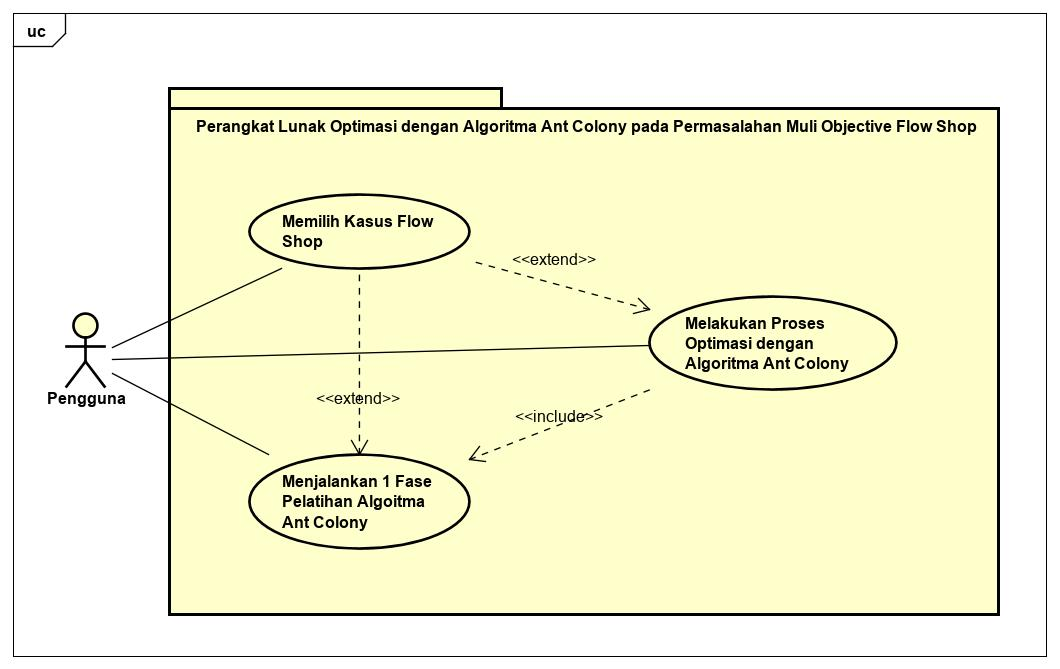
\includegraphics[scale=0.35]{UseCaseSkripsi}
		\caption[Use Case Diagram]{Use Case Diagram}
		\label{fig:usecasediagram}
	\end{figure}
	Penjelasan diagram :
	\begin{itemize}
		\item Memilih kasus Flow Shop\\
		Pengguna dapat memilih kasus flow shop yang ingin dicari hasil optimalnya. Kasus
		tersebut akan dijabarkan dalam sebuah file teks dengan format penulisan tertentu. Pengguna
		dapat memilih salah satu file teks tersebut sebagai kasus flow shop yang ingin dicari
		hasil optimalnya. Pengguna hanya dapat melakukan proses optimisasi dengan menggunakan
		algoritma ant colony setelah pengguna memilih kasus flow shop yang ingin dioptimisasi.
		\item Menjalankan 1 fase pelatihan algoritma ant colony\\
		Pengguna dapat menjalankan 1 kali fase pelatihan dari algoritma ant colony. Proses pelatihan
		ini akan mengembalikan informasi mengenai hasil optimal (makespan dan nilai utilitas mesin) yang 
		didapat pada fase pelatihan	ini.
		\item Melakukan proses optimasi dengan menggunakan algoritma ant colony\\
		Proses optimisasi ini akan menjalankan fase pelatihan algoritma ant colony secara terus 
		menerus hingga kondisi berhenti yang ditentukan tercapai. Hasil makespan dan nilai utilitas yang
		didapatkan pada setiap fase pelatihan akan ditampilkan.
	\end{itemize}
	
	\subsection{Input dan Output}
	
	Perangkat lunak akan mampu menerima data masukan dari sebuah file teks. File teks tersebut akan
	berisi informasi mengenai banyaknya mesin, banyaknya pekerjaan, waktu proses untuk setiap pekerjaan, dan 
	nilai upper beserta lower bound dari setiap kasus.
	File teks tersebut akan memiliki format penulisan tertentu, agar file teks tersebut dapat dikonversi menjadi 
	suatu kasus flow shop.
	\begin{figure}[H]
		\centering
		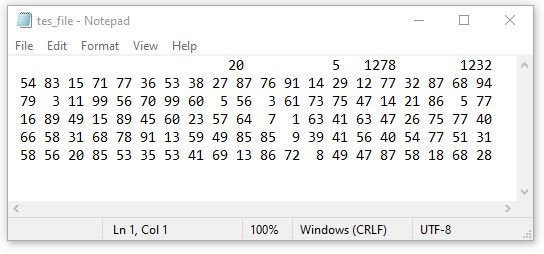
\includegraphics[scale=0.75]{InputProgram}
		\caption[Input Program]{Input Program}
		\label{fig:inputprogram}
	\end{figure}
	Gambar di atas merupakan contoh file teks yang dapat diterima oleh program yang akan dibangun. File teks 
	tersebut terdiri dari 20 pekerjaan dan 5 mesin. Penjelasan lengkap dari gambar tersebut sebagai berikut :
	\begin{enumerate}
		\item Baris pertama terdiri atas empat nilai.
		\item Nilai pertama merupakan banyaknya pekerjaan.
		\item Nilai kedua merupakan banyaknya mesin.
		\item Nilai ketiga merupakan upper bound dari suatu kasus.
		\item Nilai keempat merupakan lower bound dari suatu kasus.
		\item Baris kedua hingga akhir merupakan waktu proses untuk setiap pekerjaan.
	\end{enumerate}
	Nilai upper bound akan dianggap sebagai nilai makespan optimal / nilai makespan target yang
	ingin dicapai oleh proses optimisasi. Nilai lower bound akan dianggap sebagai nilai makespan minimal
	yang mungkin dicapai dari suatu kasus. Nilai lower bound ini akan dijadikan batas nilai
	makespan yang mungkin dihasilkan dari suatu kasus. Nilai lower bound ini akan digunakan untuk
	pengujian perangkat lunak. Jika nilai makespan yang dihasilkan lebih kecil dari nilai lower bound,
	maka kemungkinan terdapat kesalahan pada perangkat lunak.
	
	Setelah mengkonversi data masukan menjadi suatu kasus flow shop, perangkat lunak
	akan melakukan proses optimisasi. Proses optimisasi akan menghasilkan suatu solusi berupa urutan
	pengerjaan yang menghasilkan makespan yang dianggap optimal beserta nilai wait time dari setiap kasus. 
	Perangkat lunak kemudian akan
	menampilkan di layar pengguna mengenai urutan pengerjaan yang dianggap optimal, nilai
	makespan yang dihasilkan, dan nilai wait time dari suatu kasus. Perangkat lunak juga akan menampilkan 
	banyaknya pelatihan yang telah dilakukan untuk mendapat urutan pengerjaan tersebut.

	
	\subsection{Flow Chart Proses Optimasi}
	
	Proses optimisasi dengan algoritma ant colony dilakukan setelah mengkonversi data masukan menjadi
	sebuah kasus flow shop. Algoritma ant colony akan menyesuaikan diri dengan kasus flow shop yang ingin 
	dicari solusi optimalnya. Algoritma ant colony akan melakukan proses optimisasi dengan cara melakukan 
	proses pelatihan secara berulang-ulang hingga suatu kondisi berhenti tercapai. Berikut adalah flow chart 
	mengenai bagaimana perangkat lunak ini akan melakukan proses optimisasi dengan menggunakan algoritma ant colony.
	\begin{figure}[H]
		\centering
		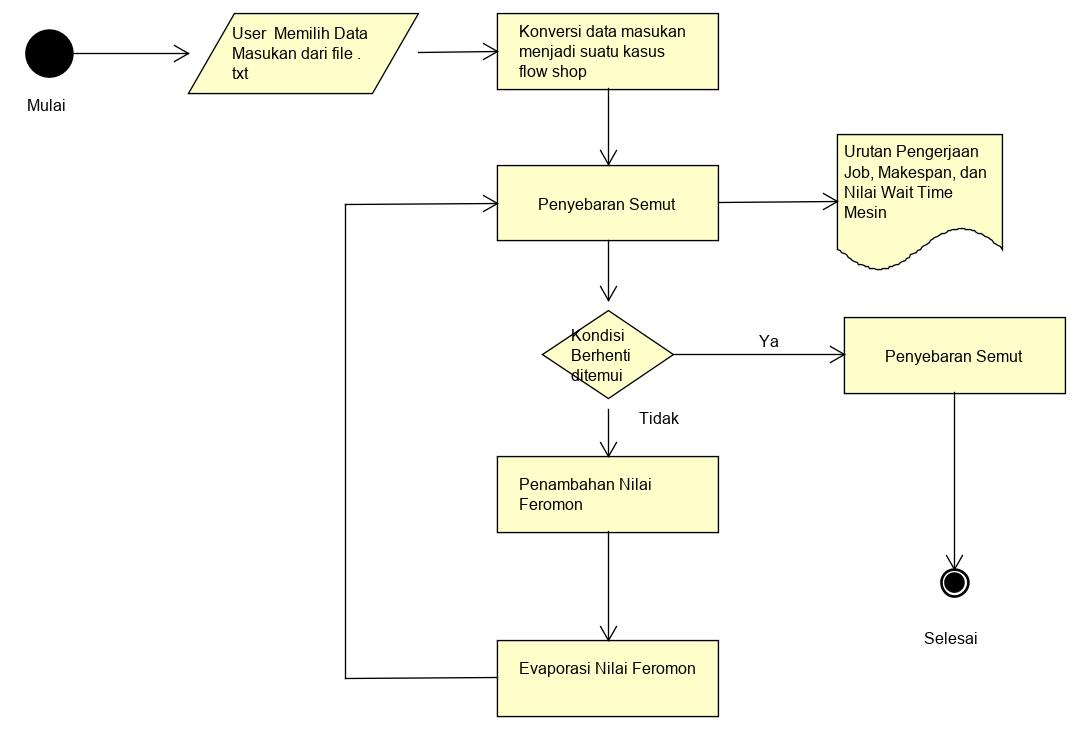
\includegraphics[scale=0.40]{FlowchartRevisi}
		\caption[Flowchart]{Flowchart Optimasi}
		\label{fig:flowchartoptimasi}
	\end{figure}
	
	
	\subsection{Diagram Kelas Secara Umum}
	
	Diagram kelas digunakan untuk memberikan gambaran mengenai kelas-kelas yang terdapat dalam
	sistem perangkat lunak yang dibangun serta hubungan antar kelasnya. Pada bab ini hanya akan ditampilkan
	diagram kelas secara umum saja. Untuk lebih detailnya akan dijelaskan pada bab selanjutnya. Diagram kelas
	tersebut sebagai berikut : 
		\begin{figure}[H]
		\centering
		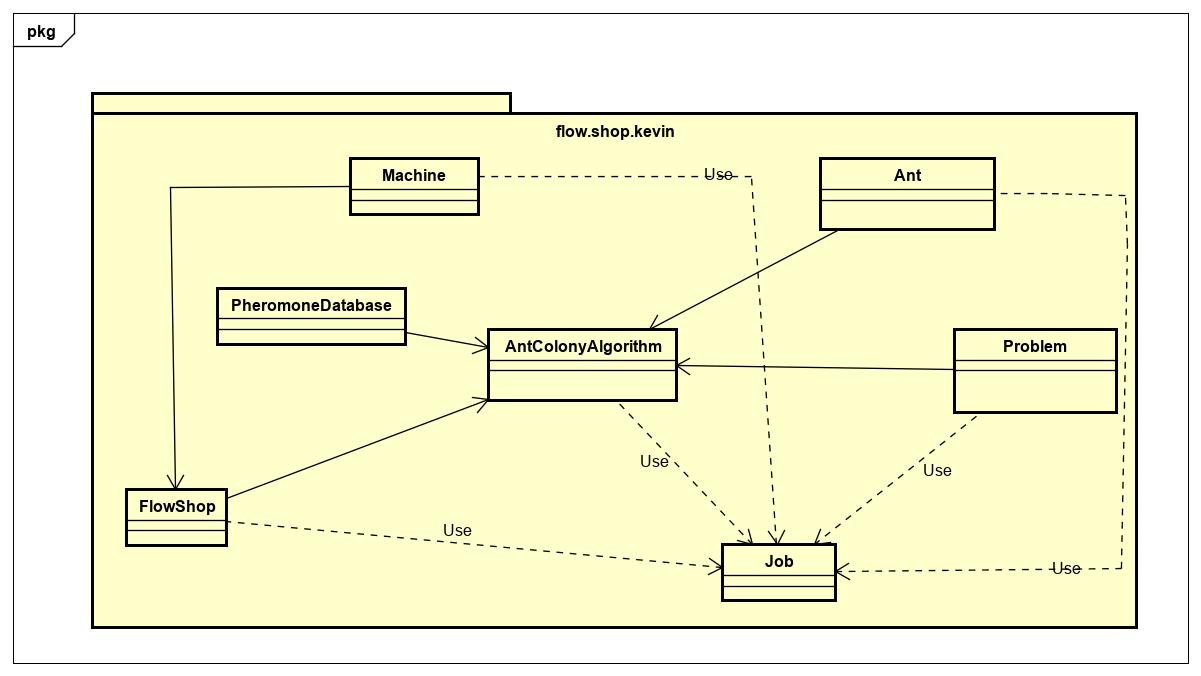
\includegraphics[scale=0.40]{ClassDiagramUmumRev}
		\caption[Diagram kelas umum]{Diagram kelas umum}
		\label{fig:diagramkelasumum}
	\end{figure}

